\documentclass[11pt,a4paper,DIV=12]{scrartcl}
\usepackage{multicol}

\makeatletter
\def\input@path{{../../../}}
\makeatother

\usepackage[sexy]{evan}
% \usepackage[sexy]{../../../evan}

% Override environment "problem" agar hanya menampilkan angka
\makeatletter
\newtheoremstyle{justnumber}
  {8pt} % space above
  {8pt} % space below
  {\normalfont} % body font
  {} % indent amount
  {\color{blue!40!black}\bfseries} % head font
  {} % punctuation after head
  {0.5em} % space after head
  {\thmnumber{#2}.\thmnote{ (\small #3)}} % head spec (hanya angka dan note)

% Hapus definisi problem lama di dalam makeatletter agar @ terbaca
\let\problem\relax
\let\endproblem\relax
\let\c@problem\relax
\let\theproblem\relax
\makeatother

\theoremstyle{justnumber}
\newtheorem{problem}{}

\begin{document}
\title{Latihan Soal 1:
  \textit{Basic Counting}}
\author{MAN 1 Pasuruan}
\date{April 2025}
\maketitle
\section*{Pilihan Ganda}
\begin{problem}[LMNAS 2013]
  Pada suatu pesta terdapat sejumlah $a$ anak-anak, $w$ wanita dewasa, dan $l$ pria dengan $2 \leq a \leq w \leq l$. Jika setiap orang hanya berjabat tangan sekali saja, dan diketahui jumlah jabat tangan anak-anak, wanita dewasa, dan pria dengan sesamanya adalah 57, maka banyaknya total jabat tangan yang terjadi dalam pesta tersebut adalah \ldots
  \begin{multicols}{5}
    \begin{enumerate}
      \item[(a)] 180
      \item[(b)] 171
      \item[(c)] 174
      \item[(d)] 178
      \item[(e)] 173
    \end{enumerate}
  \end{multicols}
\end{problem}

\begin{problem}[AMC 12A 2021]
  Sebuah organisasi memiliki $30$ karyawan, dengan $20$ di antaranya menggunakan komputer merek A dan $10$ lainnya menggunakan komputer merek B. Demi keamanan, komputer hanya dapat dihubungkan satu sama lain menggunakan kabel, dan kabel hanya dapat menghubungkan komputer merek A dengan komputer merek B. Karyawan dapat saling berkomunikasi jika komputer mereka terhubung langsung oleh kabel atau melalui rangkaian komputer yang saling terhubung. Awalnya, tidak ada komputer yang saling terhubung. Seorang teknisi secara acak memilih satu komputer dari masing-masing merek dan memasang kabel di antara keduanya, dengan syarat belum ada kabel yang menghubungkan pasangan tersebut. Teknisi berhenti ketika semua karyawan sudah dapat saling berkomunikasi. Berapa banyak maksimum kabel yang mungkin digunakan?

  \begin{multicols}{5}
    \begin{enumerate}
      \item[(A)] 190
      \item[(B)] 191
      \item[(C)] 192
      \item[(D)] 195
      \item[(E)] 196
    \end{enumerate}
  \end{multicols}
\end{problem}

\begin{problem}[AMC 12B 2025]
  Sebuah lingkaran dibagi menjadi 6 sektor dengan ukuran yang berbeda. Kemudian 2 sektor diwarnai merah, 2 diwarnai hijau, dan 2 diwarnai biru sehingga tidak ada dua sektor yang bertetangga memiliki warna yang sama. Salah satu pewarnaan ditunjukkan pada gambar di bawah ini.
  \begin{center}
    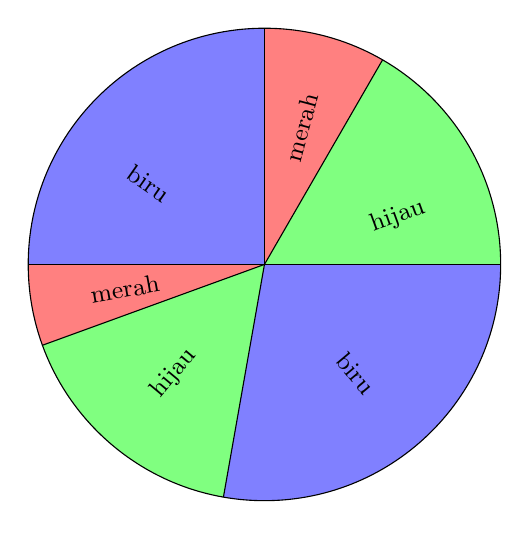
\begin{tikzpicture}
      \def\r{3}

      % Sudut pembagi sektor (tidak sama besar)
      \def\a{0}
      \def\b{60}
      \def\c{90}
      \def\d{180}
      \def\e{200}
      \def\f{260}
      \def\g{360}

      % Gambar sektor
      \fill[green!50]   (0,0) -- (\a:\r) arc(\a:\b:\r) -- cycle;
      \fill[red!50] (0,0) -- (\b:\r) arc(\b:\c:\r) -- cycle;
      \fill[blue!50]  (0,0) -- (\c:\r) arc(\c:\d:\r) -- cycle;
      \fill[red!50]   (0,0) -- (\d:\r) arc(\d:\e:\r) -- cycle;
      \fill[green!50] (0,0) -- (\e:\r) arc(\e:\f:\r) -- cycle;
      \fill[blue!50]  (0,0) -- (\f:\r) arc(\f:\g:\r) -- cycle;

      % Garis batas
      \draw (0,0) circle (\r);
      \foreach \angle in {\a,\b,\c,\d,\e,\f}
        {
          \draw (0,0) -- (\angle:\r);
        }

      % Label warna (opsional)
      \node[rotate=20] at (20:1.8)  {\small hijau};
      \node[rotate=75] at (75:1.8)  {\small merah};
      \node[rotate=-35] at (145:1.8) {\small biru};
      \node[rotate=10] at (190:1.8) {\small merah};
      \node[rotate=50] at (230:1.8) {\small hijau};
      \node[rotate=-50] at (310:1.8) {\small biru};
    \end{tikzpicture}
  \end{center}
  Banyaknya cara pewarnaan yang berbeda adalah \ldots

  \begin{multicols}{5}
    \begin{enumerate}
      \item[(A)] 12
      \item[(B)] 16
      \item[(C)] 18
      \item[(D)] 24
      \item[(E)] 28
    \end{enumerate}
  \end{multicols}
\end{problem}

\begin{problem}[AMC 12B 2024]
  Bola bernomor $1, 2, 3, \ldots$ dimasukkan ke dalam 5 kotak yang diberi label $A, B, C, D,$ dan $E$ dengan prosedur berikut. Bola 1 dimasukkan ke kotak $A$, dan bola 2 serta 3 dimasukkan ke kotak $B$. Tiga bola berikutnya dimasukkan ke kotak $C$, empat bola berikutnya ke kotak $D$, dan seterusnya, kembali ke kotak $A$ setelah bola dimasukkan ke kotak $E$. (Sebagai contoh, bola 22, 23, \ldots, 28 dimasukkan ke kotak $B$ pada langkah ke-7 dari proses ini.) Pada kotak manakah bola 2024 dimasukkan?
\end{problem}

\begin{problem}[OMITS 2021]
  Misal diberikan $n$ kotak berukuran $1 \times 1$ sedemikian hingga disusun menjadi suatu bentuk $n \times 1$. Jika $C_n$ menyatakan banyak cara menyusun kotak $n \times 1$ dengan ubin berukuran $1 \times 1$ atau $2 \times 1$, maka nilai dari
  \[
    \frac{1}{n} \left\lfloor \frac{(n+1)C_n}{nC_{n+3} - 2nC_{n+1}} \right\rfloor
  \]
  untuk $n \geq 2$ adalah \ldots

  \begin{multicols}{3}
    \begin{enumerate}
      \item[(a)] $\dfrac{1}{n}$
      \item[(b)] $1 - \dfrac{1}{n}$
      \item[(c)] $1 + \dfrac{1}{n}$
      \item[(d)] $\dfrac{2}{n}$
      \item[(e)] $2 + \dfrac{1}{n}$
    \end{enumerate}
  \end{multicols}
\end{problem}

\section*{Isian Singkat}
\begin{problem}[OSK 2020]
  Sebuah papan catur persegi panjang berukuran $3 \times 20$ akan ditutupi dengan 20 tromino seperti pada gambar di bawah ini sehingga seluruh papan catur tertutupi oleh seluruh tromino dan tidak ada tromino yang tumpang-tindih.
  \begin{center}
    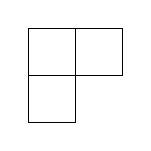
\begin{tikzpicture}[scale=0.6]
      \draw (0,0) rectangle (1,1);
      \draw (1,0) rectangle (2,1);
      \draw (0,-1) rectangle (1,0);
    \end{tikzpicture}
  \end{center}
  Banyaknya cara untuk melakukan hal tersebut adalah \ldots
\end{problem}

\begin{problem}[OSK 2021]
  Suatu komite yang terdiri dari beberapa anggota hendak menghadiri 40 rapat. Diketahui bahwa setiap rapat dihadiri tepat 10 anggota komite dan setiap dua anggota menghadiri rapat bersama paling banyak satu kali. Banyaknya anggota komite terkecil yang mungkin adalah \ldots
\end{problem}

\begin{problem}[KTOM Juni 2021]
  Sekolah KTOM mengirimkan dua belas siswanya untuk mengikuti lomba cerdas cermat dan debat. Diketahui kedua belas siswa tersebut dibagi menjadi empat tim dengan sama rata, dimana dua tim diikutkan pada lomba cerdas cermat serta dua tim sisanya diikutkan pada lomba debat. Apabila Jessen dan Valen adalah dua siswa paling imba dari kedua belas siswa tersebut, sehingga mereka tidak boleh dimasukkan dalam satu tim yang sama, tentukan banyak cara untuk membuat keempat tim tersebut.

  \noindent\textit{Catatan: Dua tim pada satu lomba yang sama memiliki derajat yang sama.}
\end{problem}


\begin{problem}[OSP 2015]
  Dalam suatu pesta, setiap pria berjabat tangan dengan pria lain hanya sekali. Demikian juga, setiap wanita hanya berjabat tangan sekali dengan wanita lain yang hadir dalam pesta tersebut. Tidak ada yang berjabat tangan antara pria dan wanita dalam pesta tersebut. Jika banyaknya pria yang hadir dalam pesta lebih banyak dari wanita dan jumlah jabat tangan antara pria atau wanita ada 7 jabat tangan. Banyaknya pria yang hadir dalam pesta tersebut adalah \ldots
\end{problem}


\begin{problem}[Introductory Combinatory, Brualdi]
  Berapa banyak solusi bilangan bulat dari
  \[
    x_1 + x_2 + x_3 + x_4 = 30
  \]
  yang memenuhi $x_1 \geq 2$, $x_2 \geq 0$, $x_3 \geq -5$, dan $x_4 \geq 8$?
\end{problem}

\begin{problem}[Introductory Combinatory, Brualdi]
  Dalam sebuah turnamen sepak bola yang terdiri dari 15 tim, tiga tim teratas mendapatkan piala emas, perak, dan perunggu, sedangkan tiga tim terbawah terdegradasi ke liga yang lebih rendah. Dua hasil turnamen dianggap sama jika tim yang mendapatkan piala emas, perak, dan perunggu masing-masing sama, serta tim yang terdegradasi juga sama. Berapa banyak kemungkinan hasil berbeda yang mungkin terjadi pada turnamen tersebut?
\end{problem}
\begin{problem}[102 Combinatorial  Problem]
  Seekor laba-laba memiliki satu kaus kaki dan satu sepatu untuk masing-masing dari delapan kakinya. Dalam berapa banyak urutan berbeda laba-laba tersebut dapat memakai kaus kaki dan sepatunya, dengan asumsi bahwa pada setiap kaki, kaus kaki harus dipakai sebelum sepatu?
\end{problem}
\end{document}